\documentclass[11pt,]{article}
\usepackage{lmodern}
\usepackage{amssymb,amsmath}
\usepackage{ifxetex,ifluatex}
\usepackage{fixltx2e} % provides \textsubscript
\ifnum 0\ifxetex 1\fi\ifluatex 1\fi=0 % if pdftex
  \usepackage[T1]{fontenc}
  \usepackage[utf8]{inputenc}
\else % if luatex or xelatex
  \ifxetex
    \usepackage{mathspec}
  \else
    \usepackage{fontspec}
  \fi
  \defaultfontfeatures{Ligatures=TeX,Scale=MatchLowercase}
\fi
% use upquote if available, for straight quotes in verbatim environments
\IfFileExists{upquote.sty}{\usepackage{upquote}}{}
% use microtype if available
\IfFileExists{microtype.sty}{%
\usepackage{microtype}
\UseMicrotypeSet[protrusion]{basicmath} % disable protrusion for tt fonts
}{}
\usepackage[margin=1.0in]{geometry}
\usepackage{hyperref}
\hypersetup{unicode=true,
            pdftitle={Supplementary},
            pdfborder={0 0 0},
            breaklinks=true}
\urlstyle{same}  % don't use monospace font for urls
\usepackage{graphicx,grffile}
\makeatletter
\def\maxwidth{\ifdim\Gin@nat@width>\linewidth\linewidth\else\Gin@nat@width\fi}
\def\maxheight{\ifdim\Gin@nat@height>\textheight\textheight\else\Gin@nat@height\fi}
\makeatother
% Scale images if necessary, so that they will not overflow the page
% margins by default, and it is still possible to overwrite the defaults
% using explicit options in \includegraphics[width, height, ...]{}
\setkeys{Gin}{width=\maxwidth,height=\maxheight,keepaspectratio}
\IfFileExists{parskip.sty}{%
\usepackage{parskip}
}{% else
\setlength{\parindent}{0pt}
\setlength{\parskip}{6pt plus 2pt minus 1pt}
}
\setlength{\emergencystretch}{3em}  % prevent overfull lines
\providecommand{\tightlist}{%
  \setlength{\itemsep}{0pt}\setlength{\parskip}{0pt}}
\setcounter{secnumdepth}{0}
% Redefines (sub)paragraphs to behave more like sections
\ifx\paragraph\undefined\else
\let\oldparagraph\paragraph
\renewcommand{\paragraph}[1]{\oldparagraph{#1}\mbox{}}
\fi
\ifx\subparagraph\undefined\else
\let\oldsubparagraph\subparagraph
\renewcommand{\subparagraph}[1]{\oldsubparagraph{#1}\mbox{}}
\fi

%%% Use protect on footnotes to avoid problems with footnotes in titles
\let\rmarkdownfootnote\footnote%
\def\footnote{\protect\rmarkdownfootnote}

%%% Change title format to be more compact
\usepackage{titling}

% Create subtitle command for use in maketitle
\newcommand{\subtitle}[1]{
  \posttitle{
    \begin{center}\large#1\end{center}
    }
}

\setlength{\droptitle}{-2em}

  \title{Supplementary}
    \pretitle{\vspace{\droptitle}\centering\huge}
  \posttitle{\par}
    \author{}
    \preauthor{}\postauthor{}
    \date{}
    \predate{}\postdate{}
  
\usepackage{booktabs}
\usepackage{longtable}
\usepackage{array}
\usepackage{multirow}
\usepackage[table]{xcolor}
\usepackage{wrapfig}
\usepackage{float}
\usepackage{colortbl}
\usepackage{pdflscape}
\usepackage{tabu}
\usepackage{threeparttable}
\usepackage{threeparttablex}
\usepackage[normalem]{ulem}
\usepackage{makecell}
\usepackage{caption}

\usepackage{helvet} % Helvetica font
\renewcommand*\familydefault{\sfdefault} % Use the sans serif version of the font
\usepackage[T1]{fontenc}

\usepackage[none]{hyphenat}

\usepackage{setspace}
\doublespacing
\setlength{\parskip}{1em}

\usepackage{lineno}

\usepackage{pdfpages}
\floatplacement{figure}{H} % Keep the figure up top of the page
\usepackage{booktabs}
\usepackage{longtable}
\usepackage{array}
\usepackage{multirow}
\usepackage{wrapfig}
\usepackage{float}
\usepackage{colortbl}
\usepackage{pdflscape}
\usepackage{tabu}
\usepackage{threeparttable}
\usepackage{threeparttablex}
\usepackage[normalem]{ulem}
\usepackage{makecell}
\usepackage{xcolor}

\begin{document}
\maketitle

\section{Gender representation}\label{gender-representation}

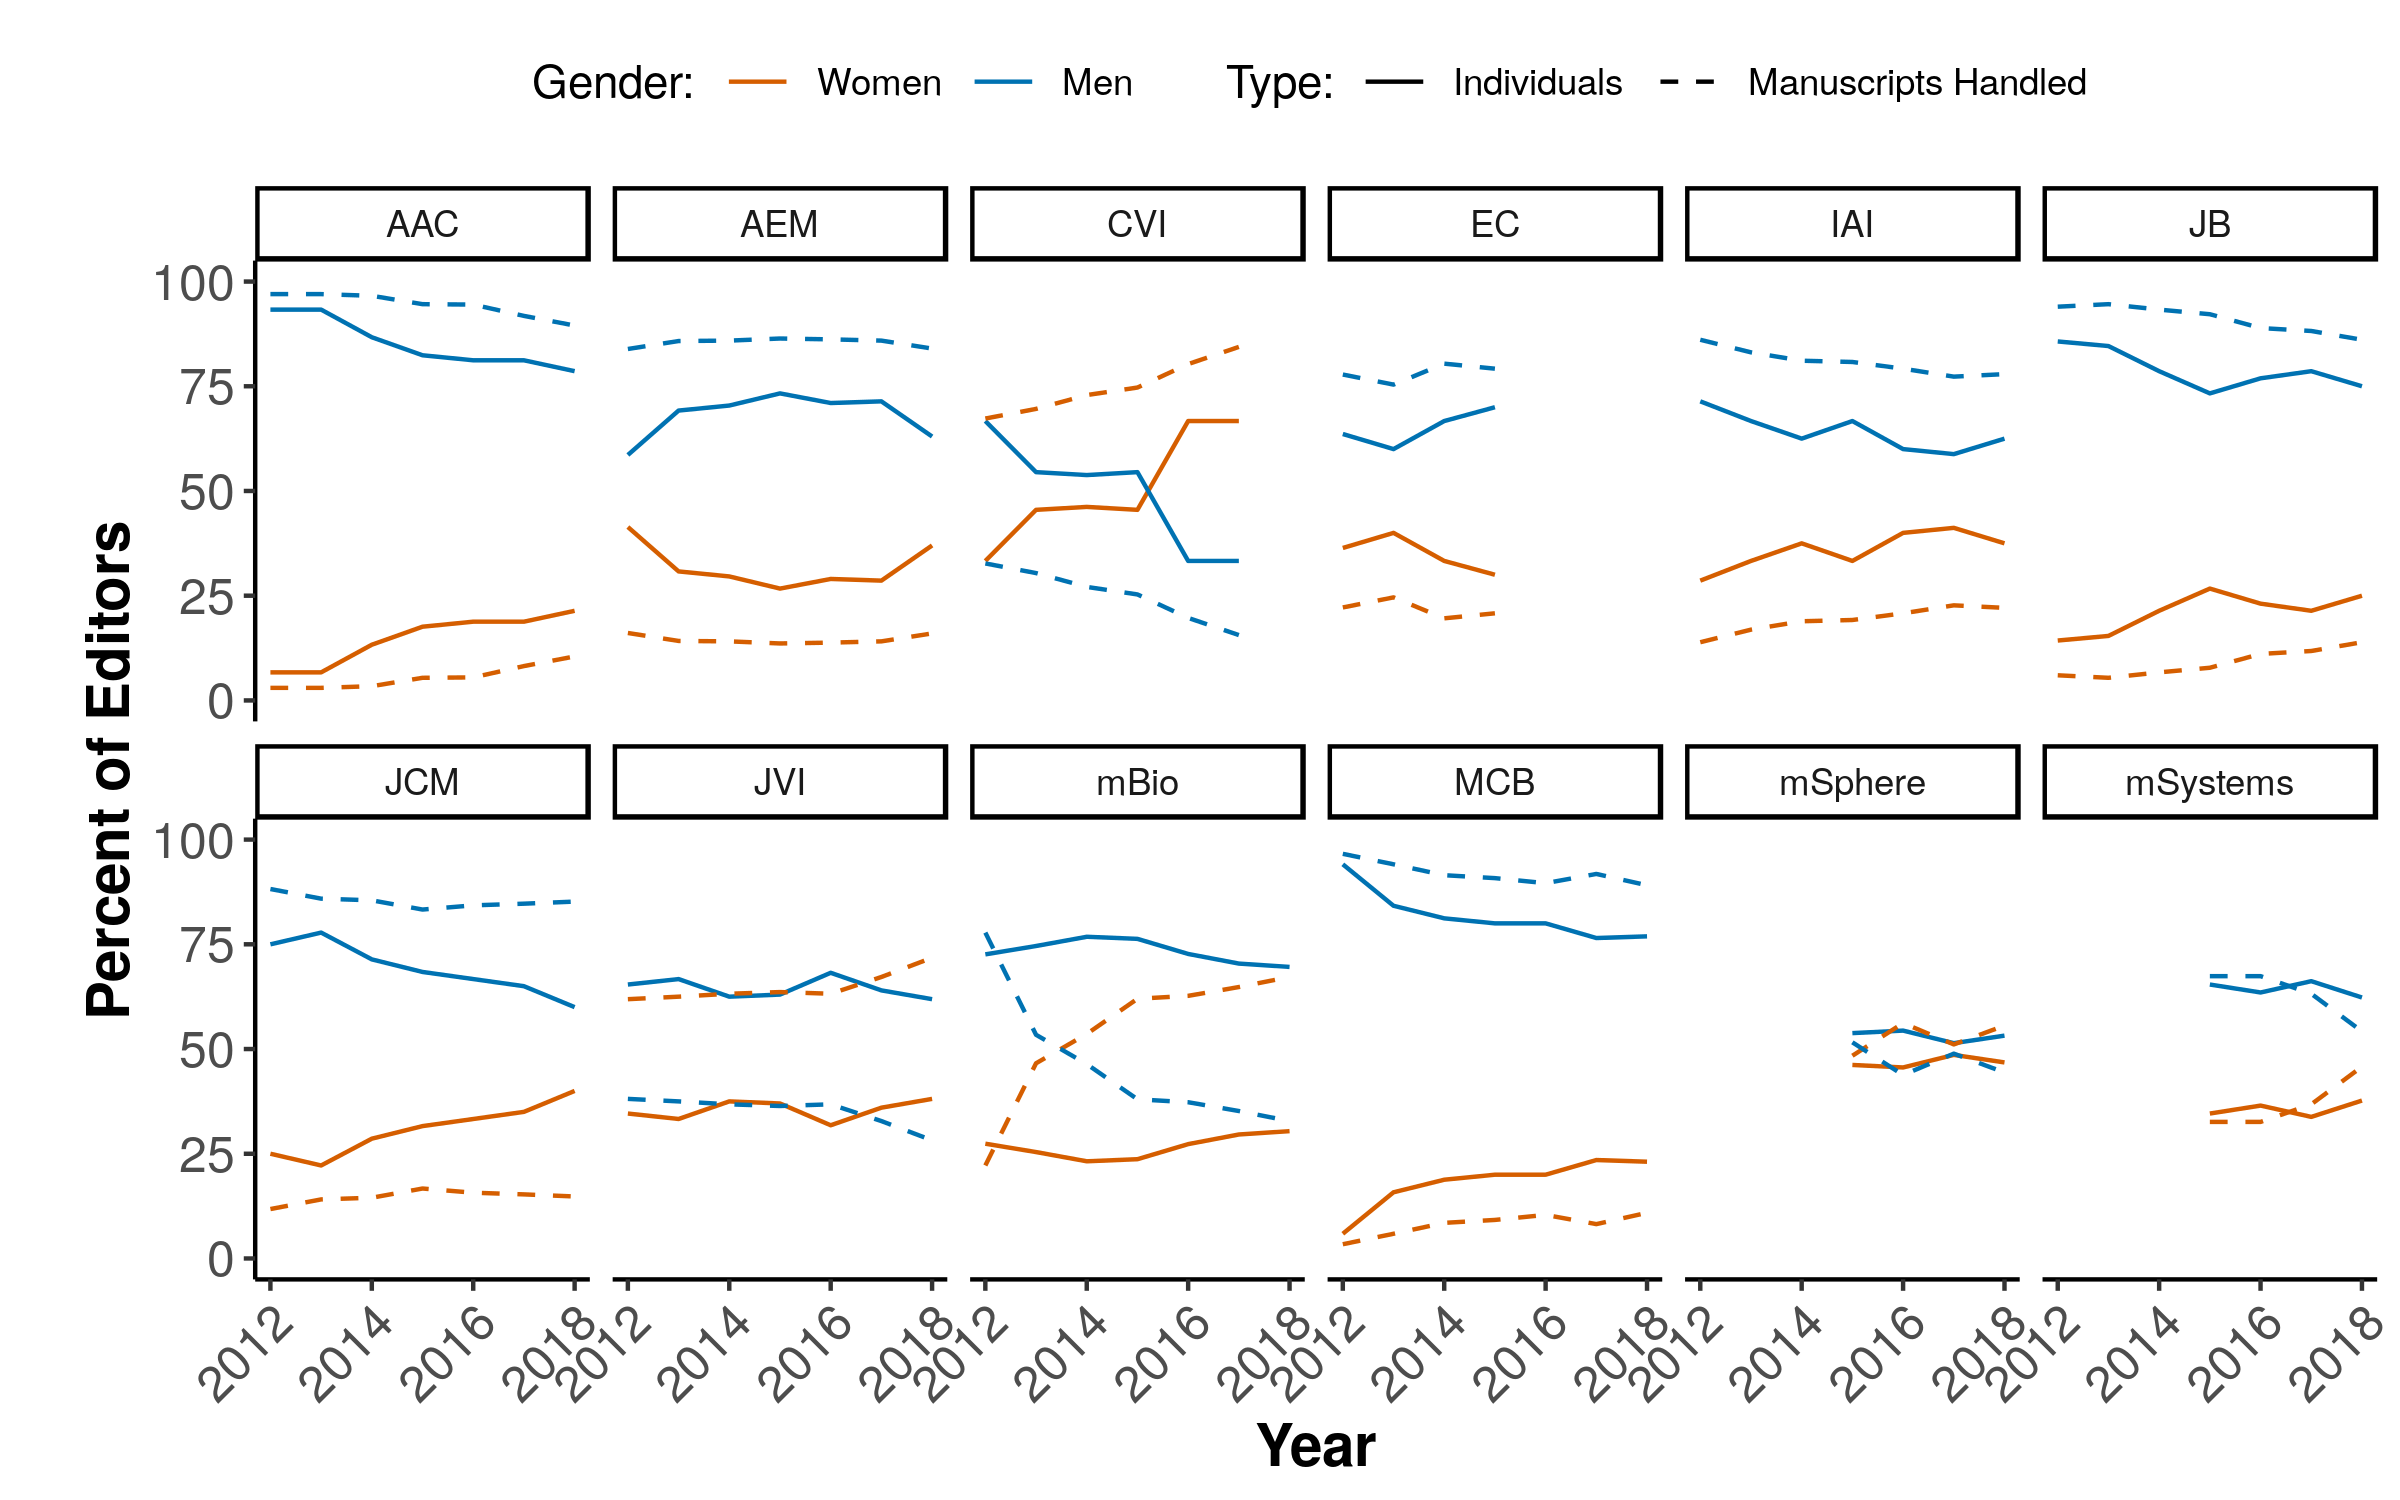
\includegraphics{Figure_S1.png}

Figure S1. The proportion of (A) potential reviewers at all ASM journals
combined, (B) reviewers at each ASM journal, (C) all submitting (dashed
line) and publishing (solid line) middle authors, and (D) all submitting
and publishing last authors by gender.

\newpage

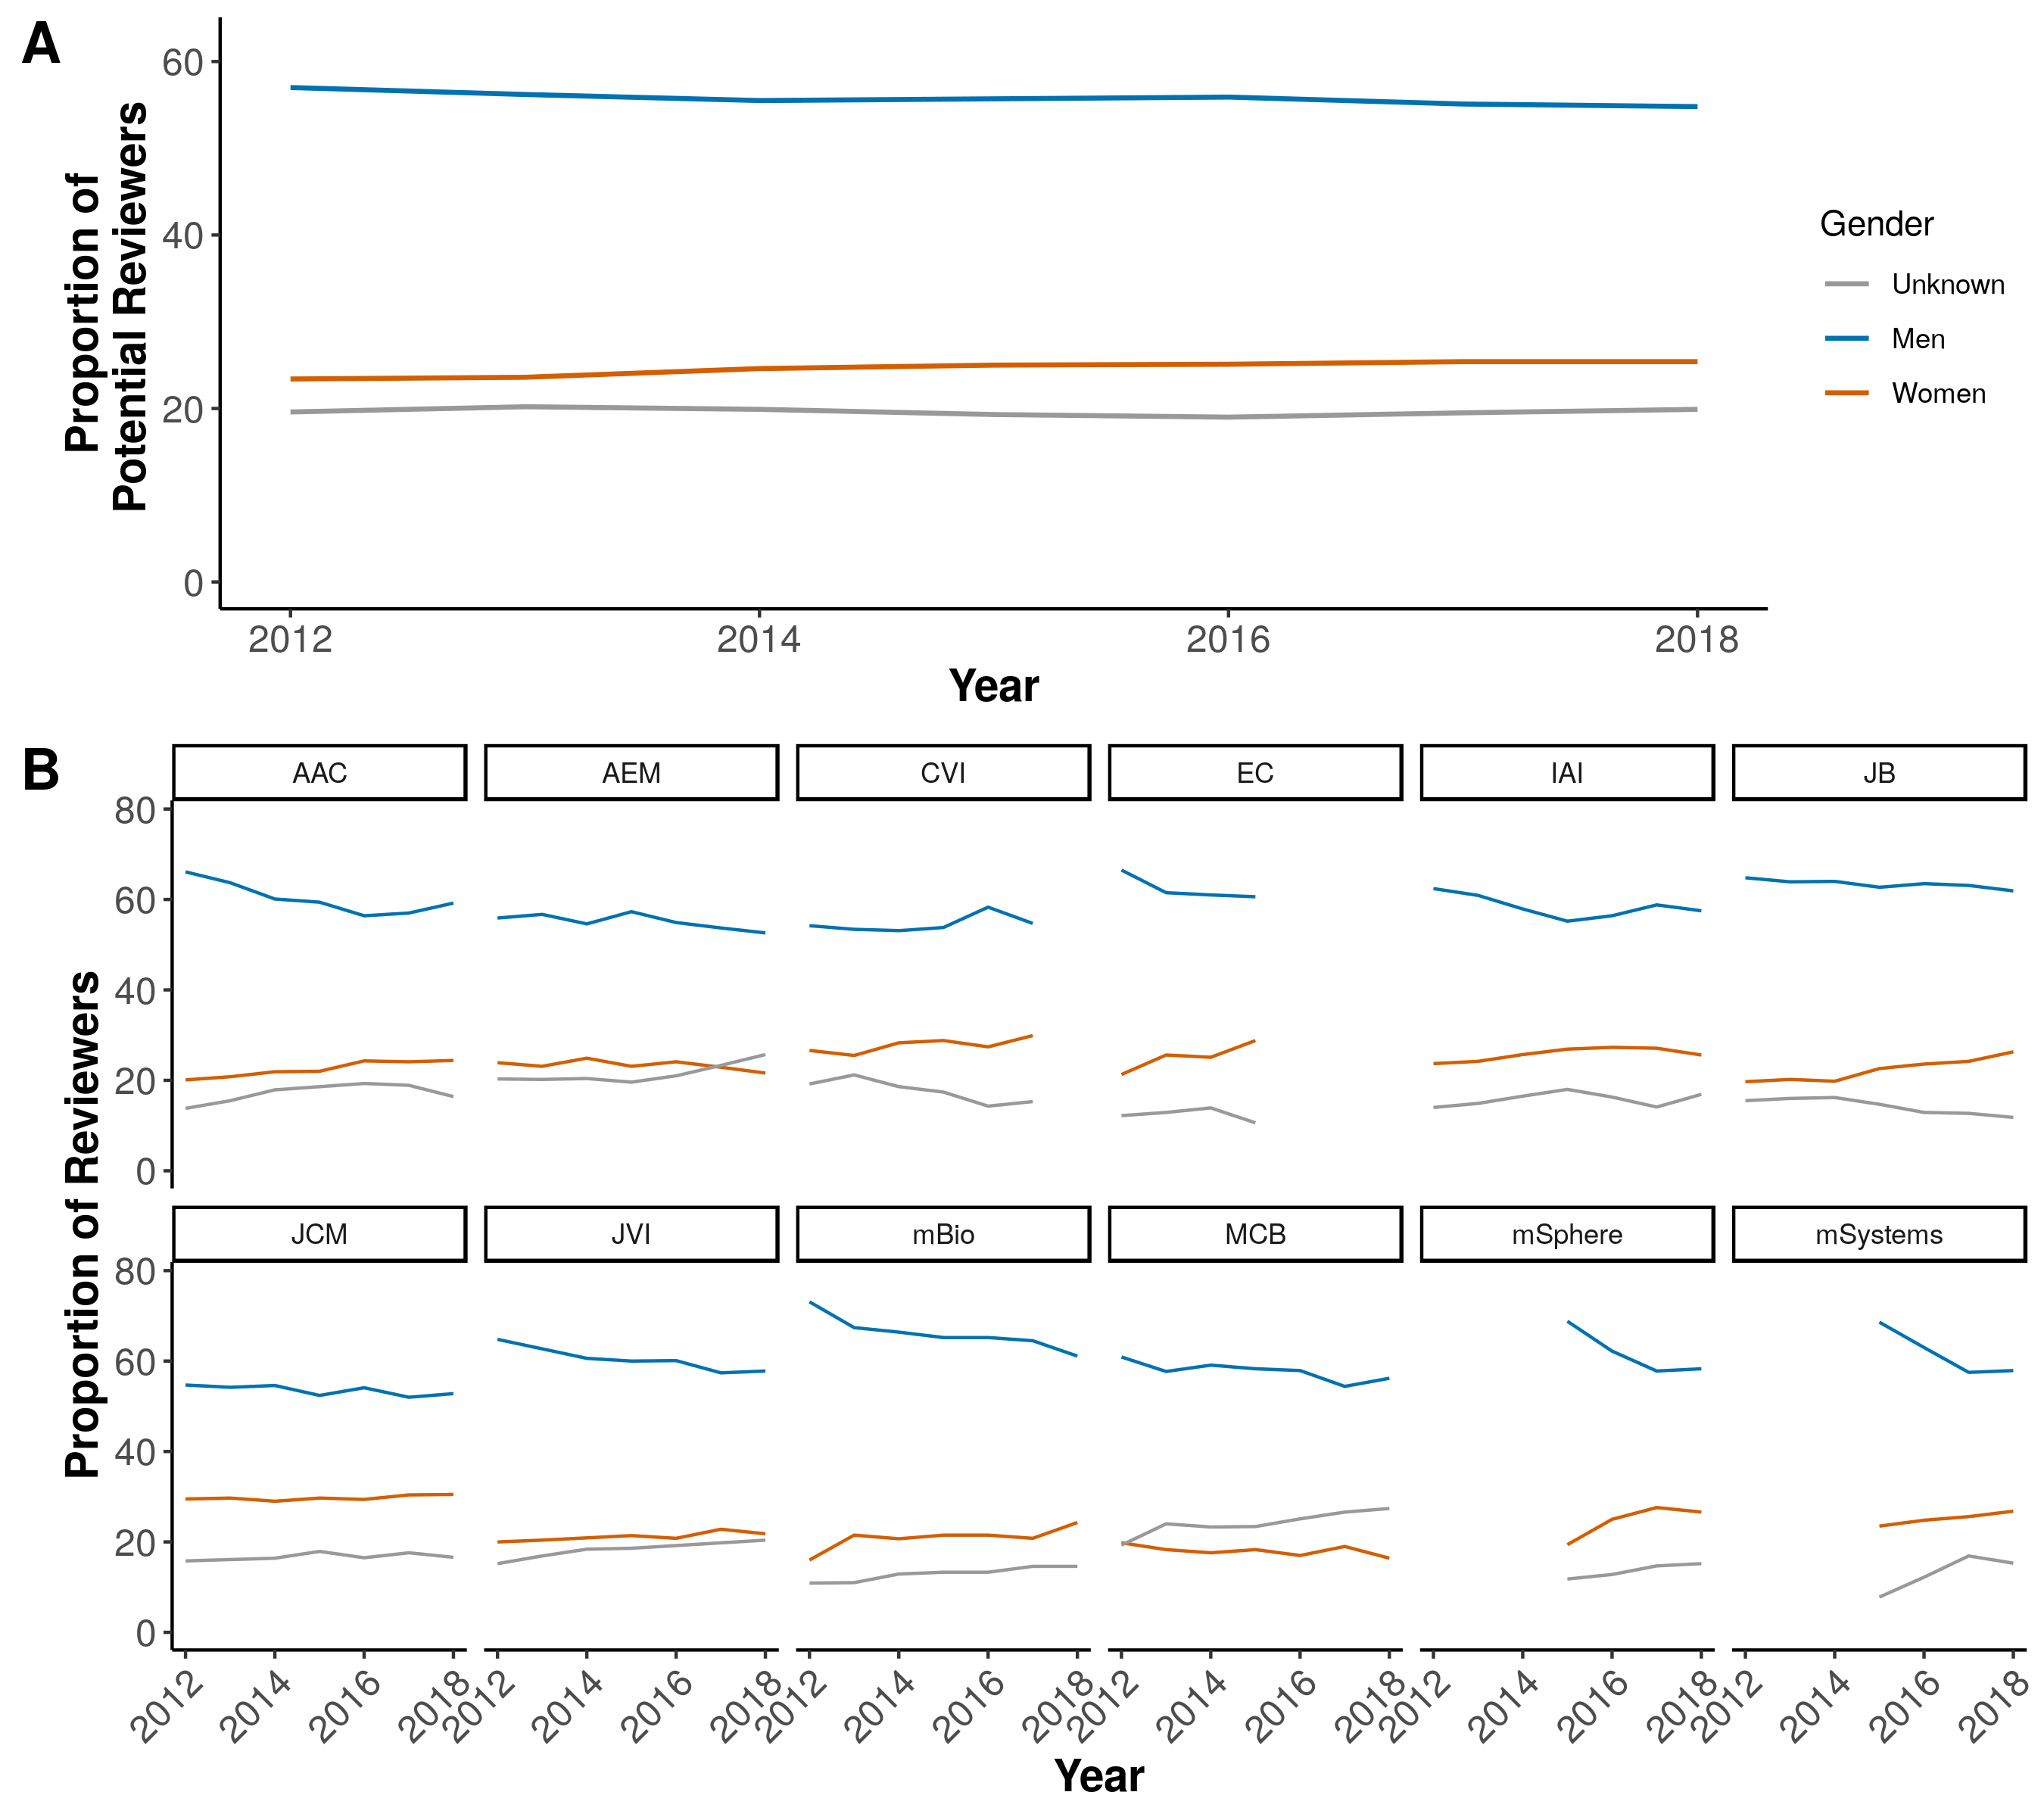
\includegraphics{Figure_S2.png} Figure S2. The proportion of all
submitting (dashed line) and publishing (solid line) (A) first and (B)
corresponding authors by gender at each ASM journal.

\newpage

\section{Gender bias}\label{gender-bias}

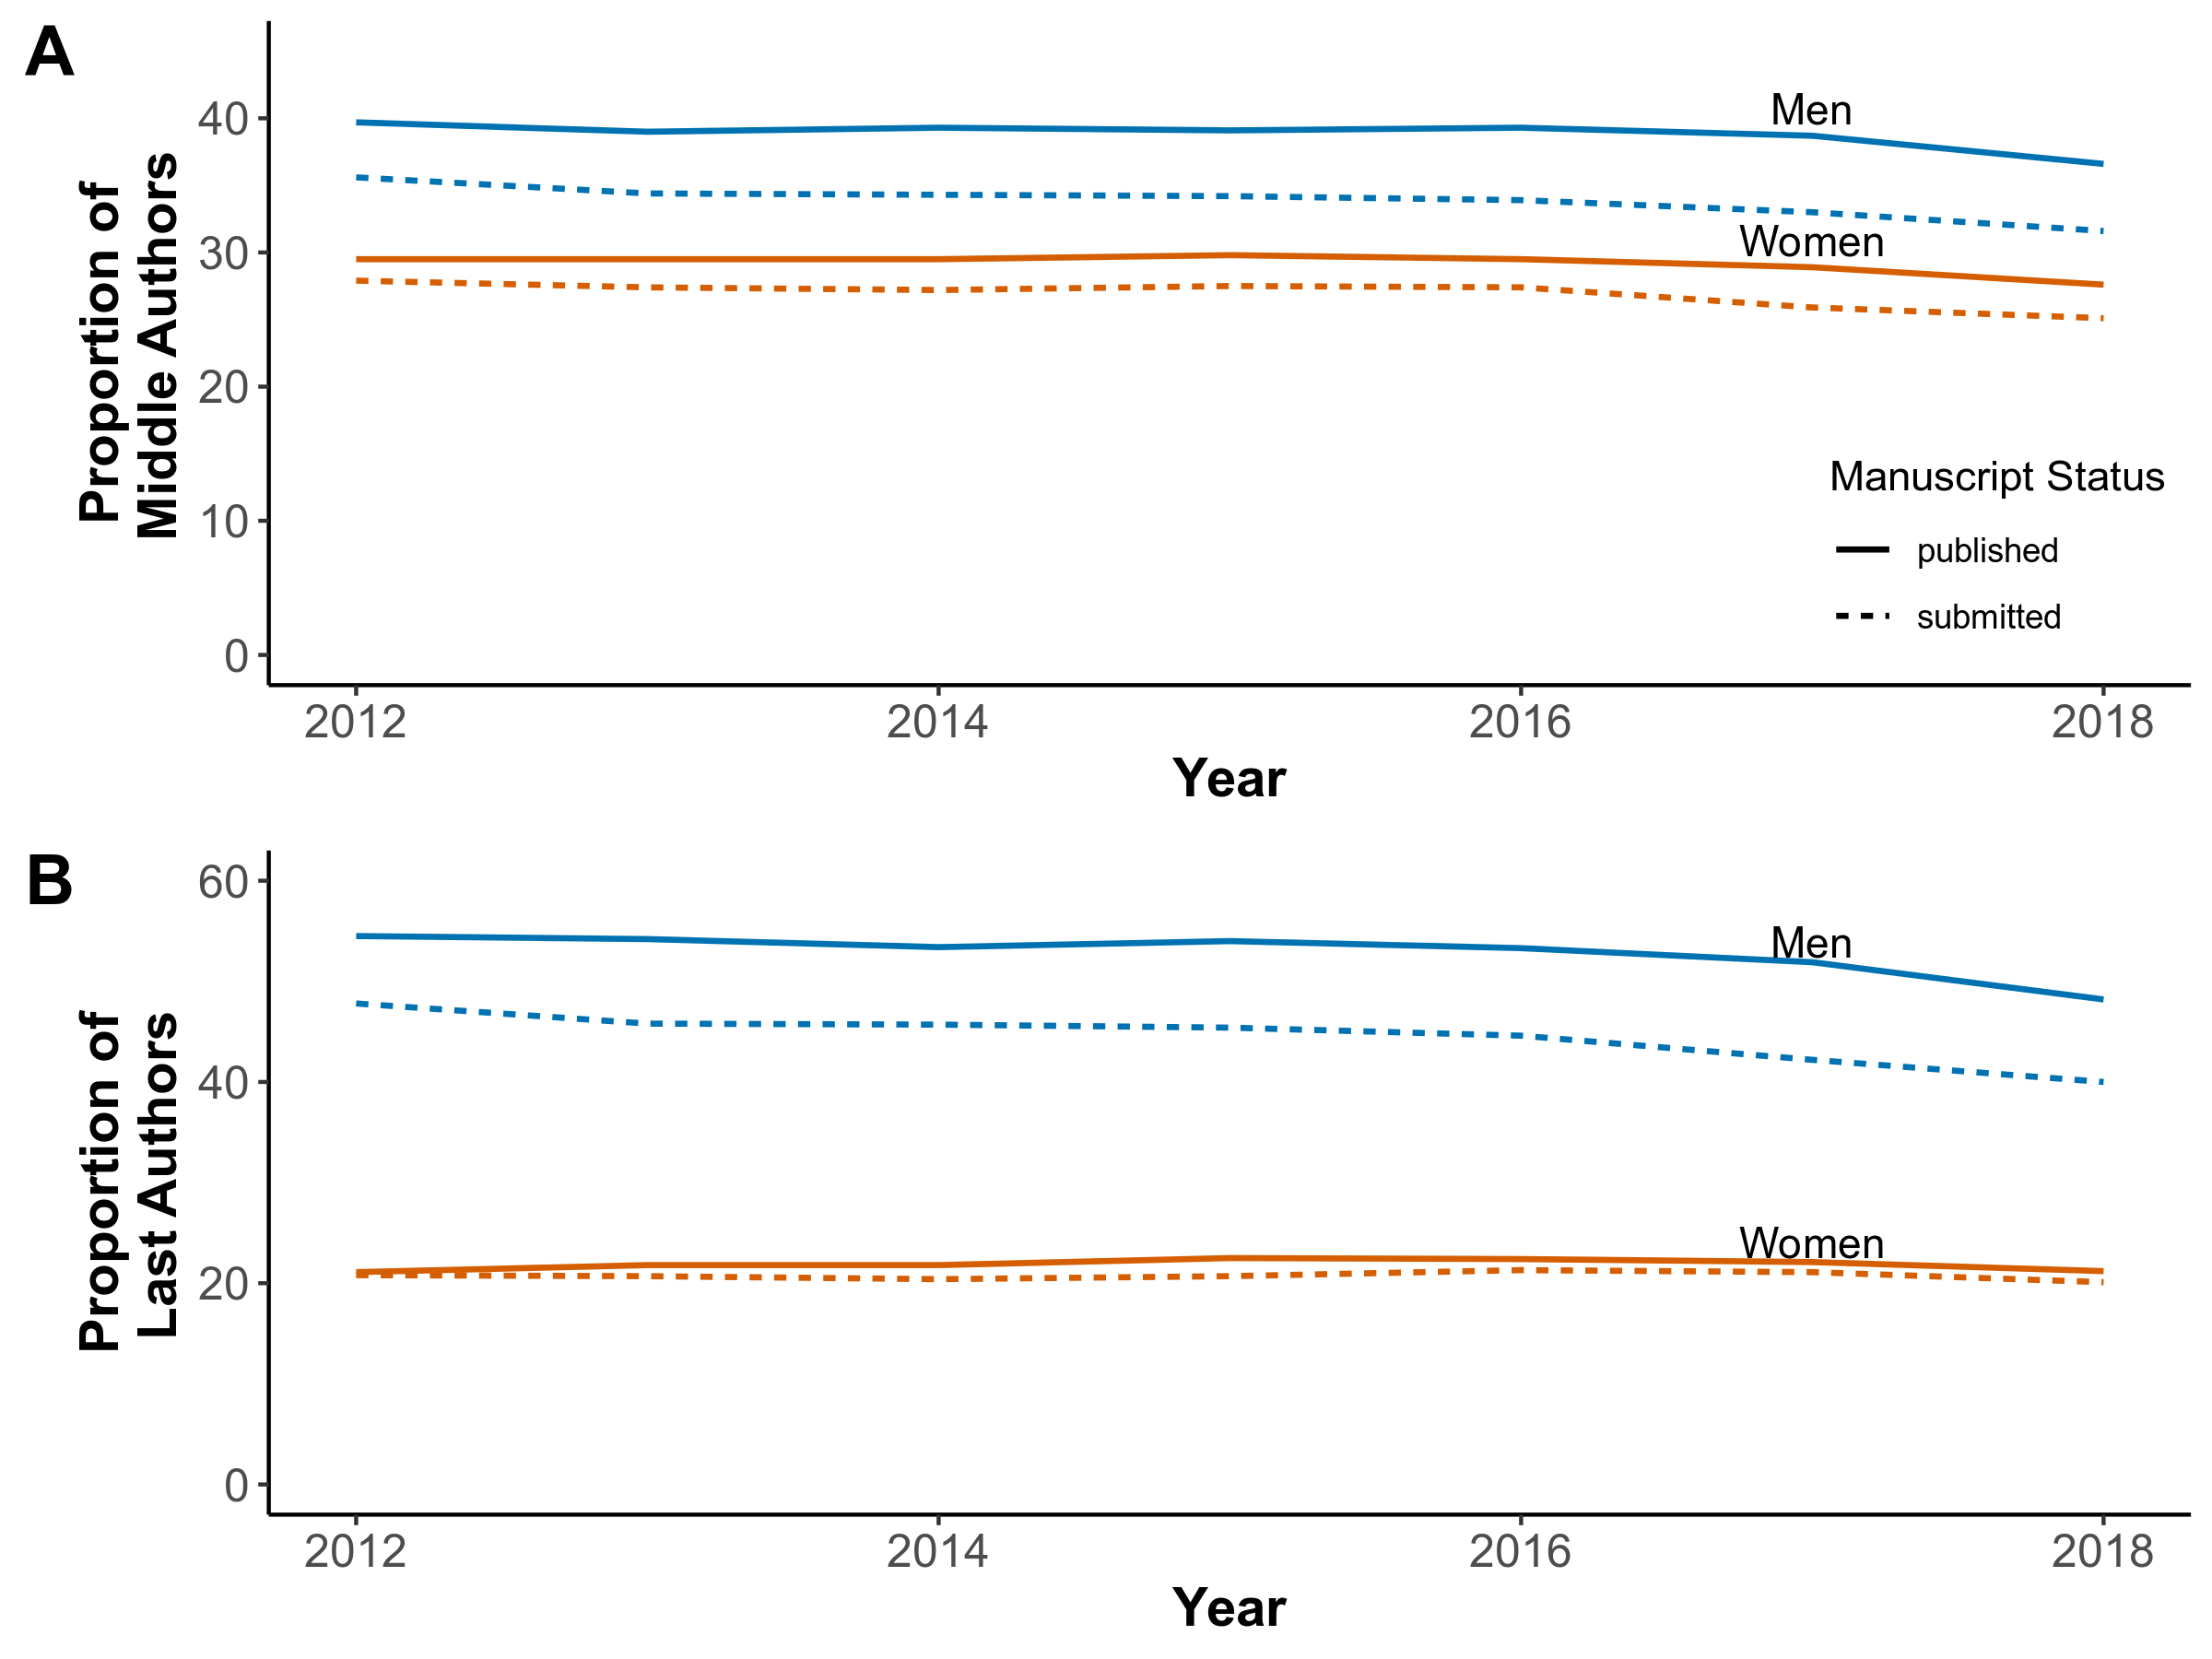
\includegraphics{Figure_S3.png}

Figure S3. Comparison of time to final decision and impact by gender.**
The number days (A) between when a manuscript is initally submitted then
finally published and (B) that a manuscript spends in the ASM peer
review system. How the impact of papers published by men (blue) versus
women (orange) vary according to (C) cites and (D) total reads. Citation
data includes articles published between 36 and 48 months prior to
August 2018. Total reads includes both HTML and PDF online views for
articles published between 12 and 24 months prior to August 2018. Impact
data are divided by the number of months published.

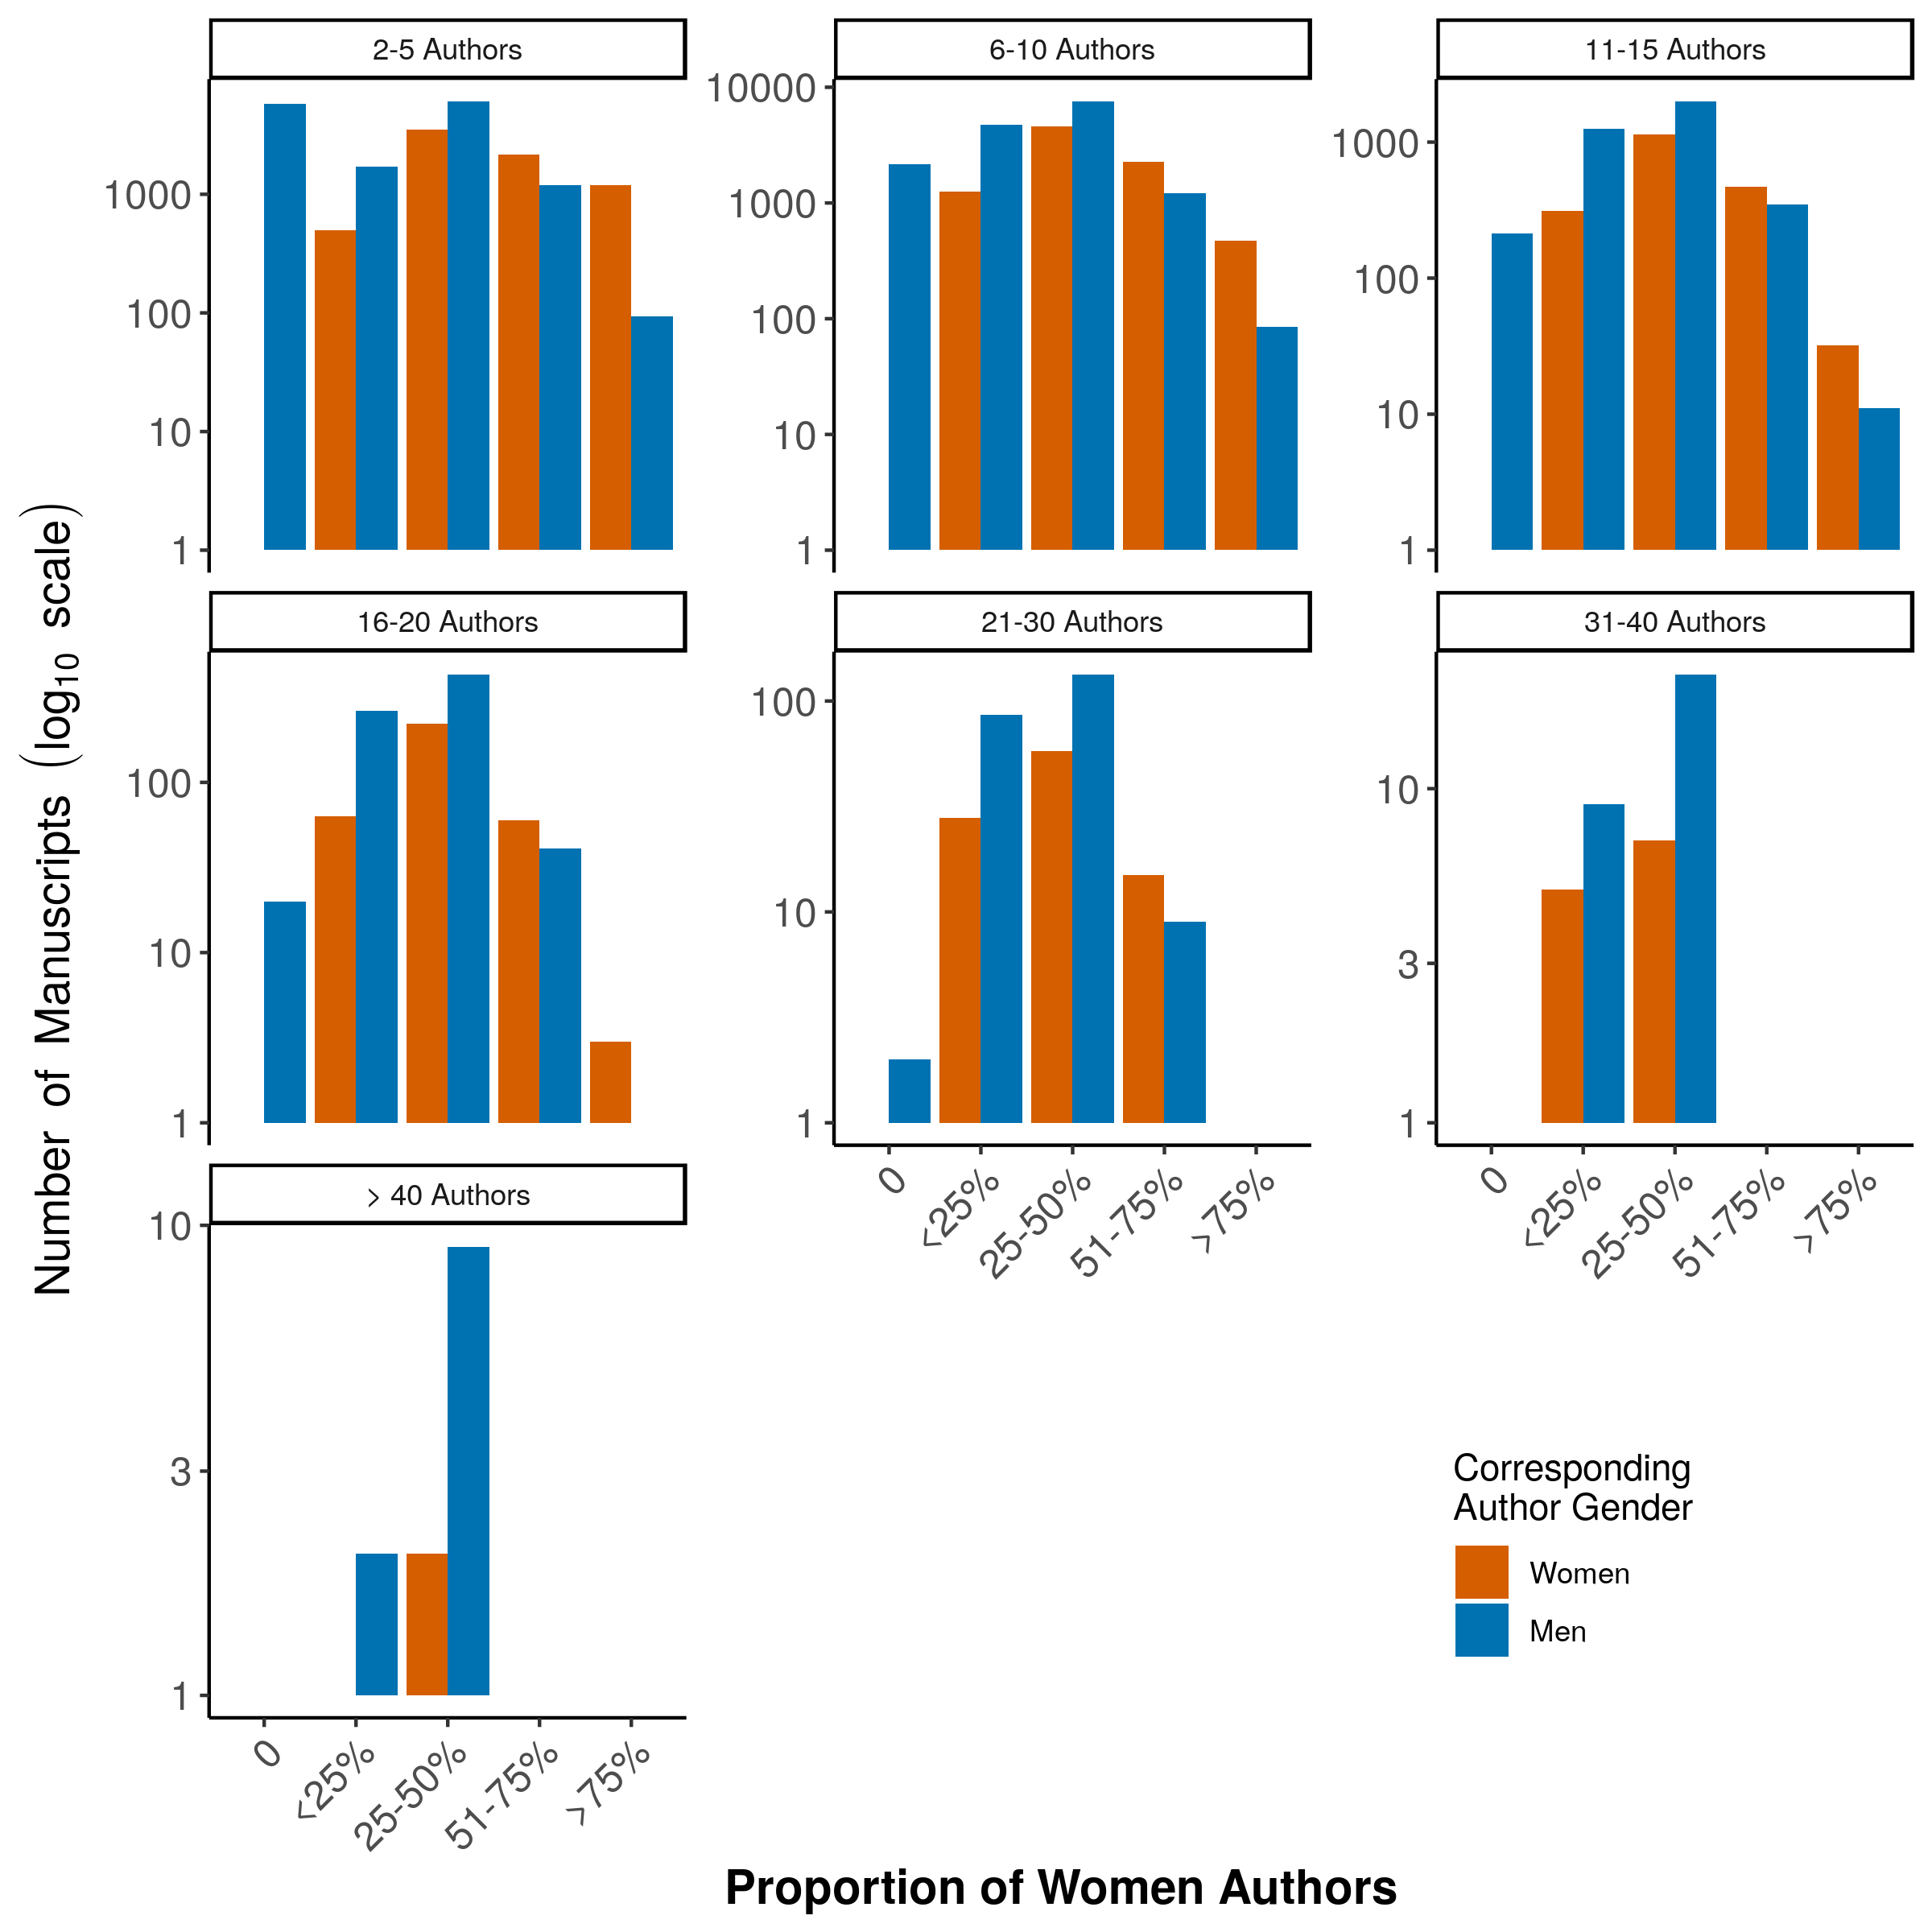
\includegraphics{Figure_S4.png}

Figure S4. Difference in acceptance and rejections by institution type.

\newpage

\subsection{Gender prediction and
assignment}\label{gender-prediction-and-assignment}

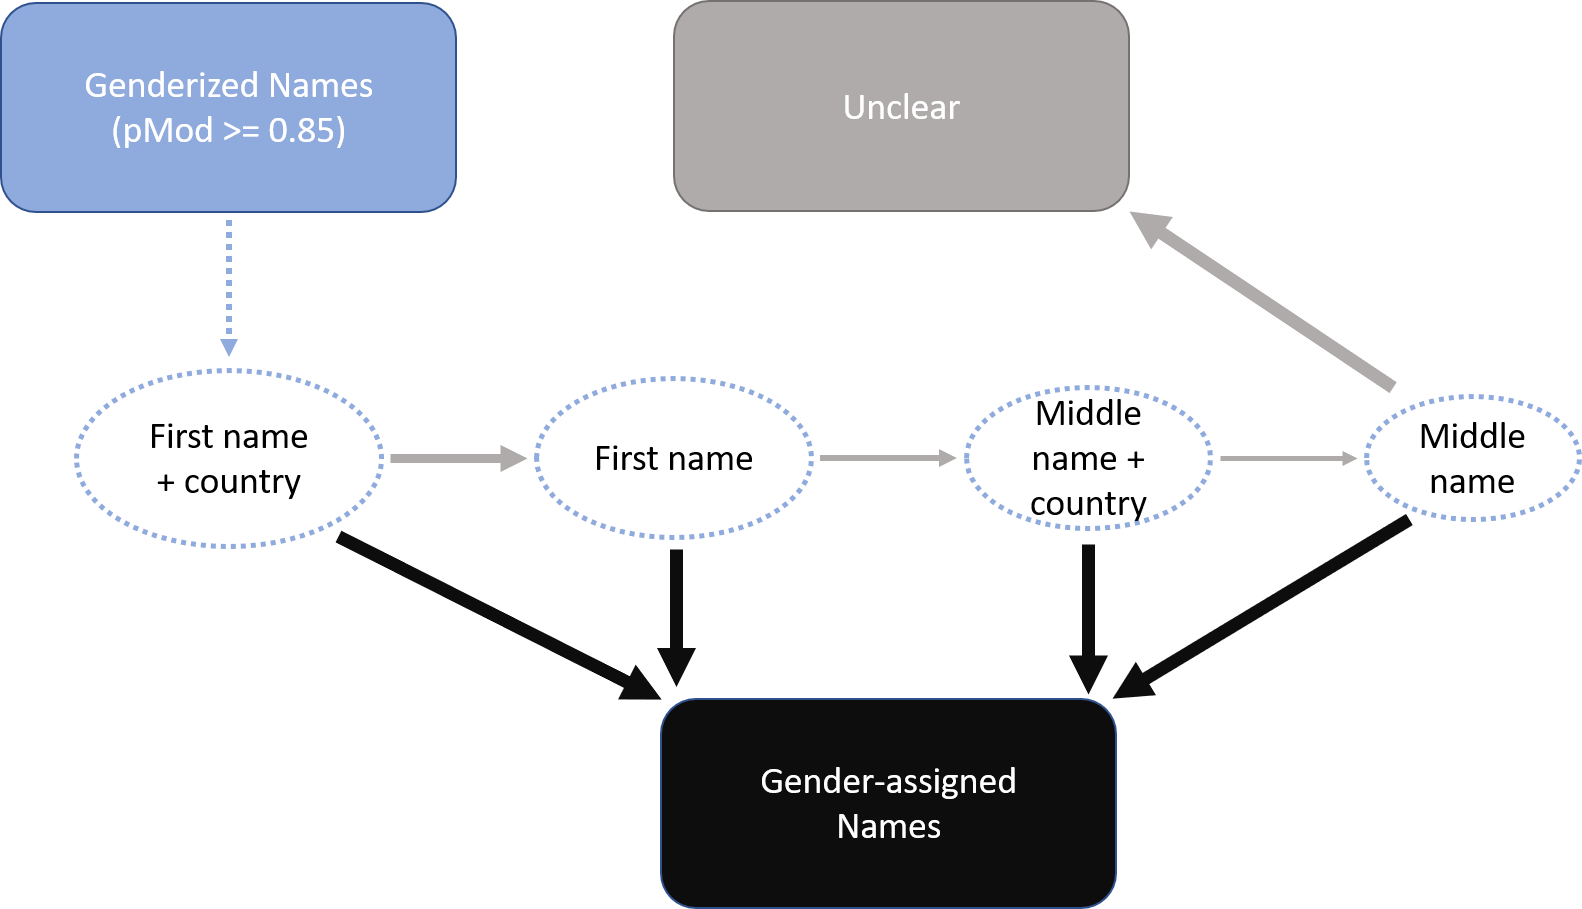
\includegraphics{genderize_method.png}

Figure S5. Schematic of gender prediction and assignment.

\newpage

\subsection{Validating gender
analysis}\label{validating-gender-analysis}

Table S1. sensitivity/specificity/accuracy of genderize thresholds.
Bolded text denotes the accuracy of the threshold used in all further
analyses.

\begin{table}[H]
\centering
\begin{tabular}{l|r|r|l|r|r|l}
\hline
\multicolumn{1}{c|}{ } & \multicolumn{3}{c|}{First Names} & \multicolumn{3}{c}{Plus Country Data} \\
\cline{2-4} \cline{5-7}
Measure & p0.5 & p0.85 & pmod0.85 & p0.5 & p0.85 & pmod0.85\\
\hline
Sensitivity & 0.8943 & 0.9516 & \cellcolor{white}{0.971} & 0.9055 & 0.9471 & \cellcolor{white}{0.9669}\\
\hline
Specificity & 0.9339 & 0.9593 & \cellcolor{white}{0.972} & 0.9265 & 0.9553 & \cellcolor{white}{0.9727}\\
\hline
Accuracy & 0.9110 & 0.9549 & \textbf{0.9714} & 0.9146 & 0.9507 & \textbf{0.9695}\\
\hline
\end{tabular}
\end{table}

\vspace{40mm}


\includegraphics{impact_equation.png}

Figure S6. Equation for calculating negative bias by genderize. C
indicates an individual country.

\newpage

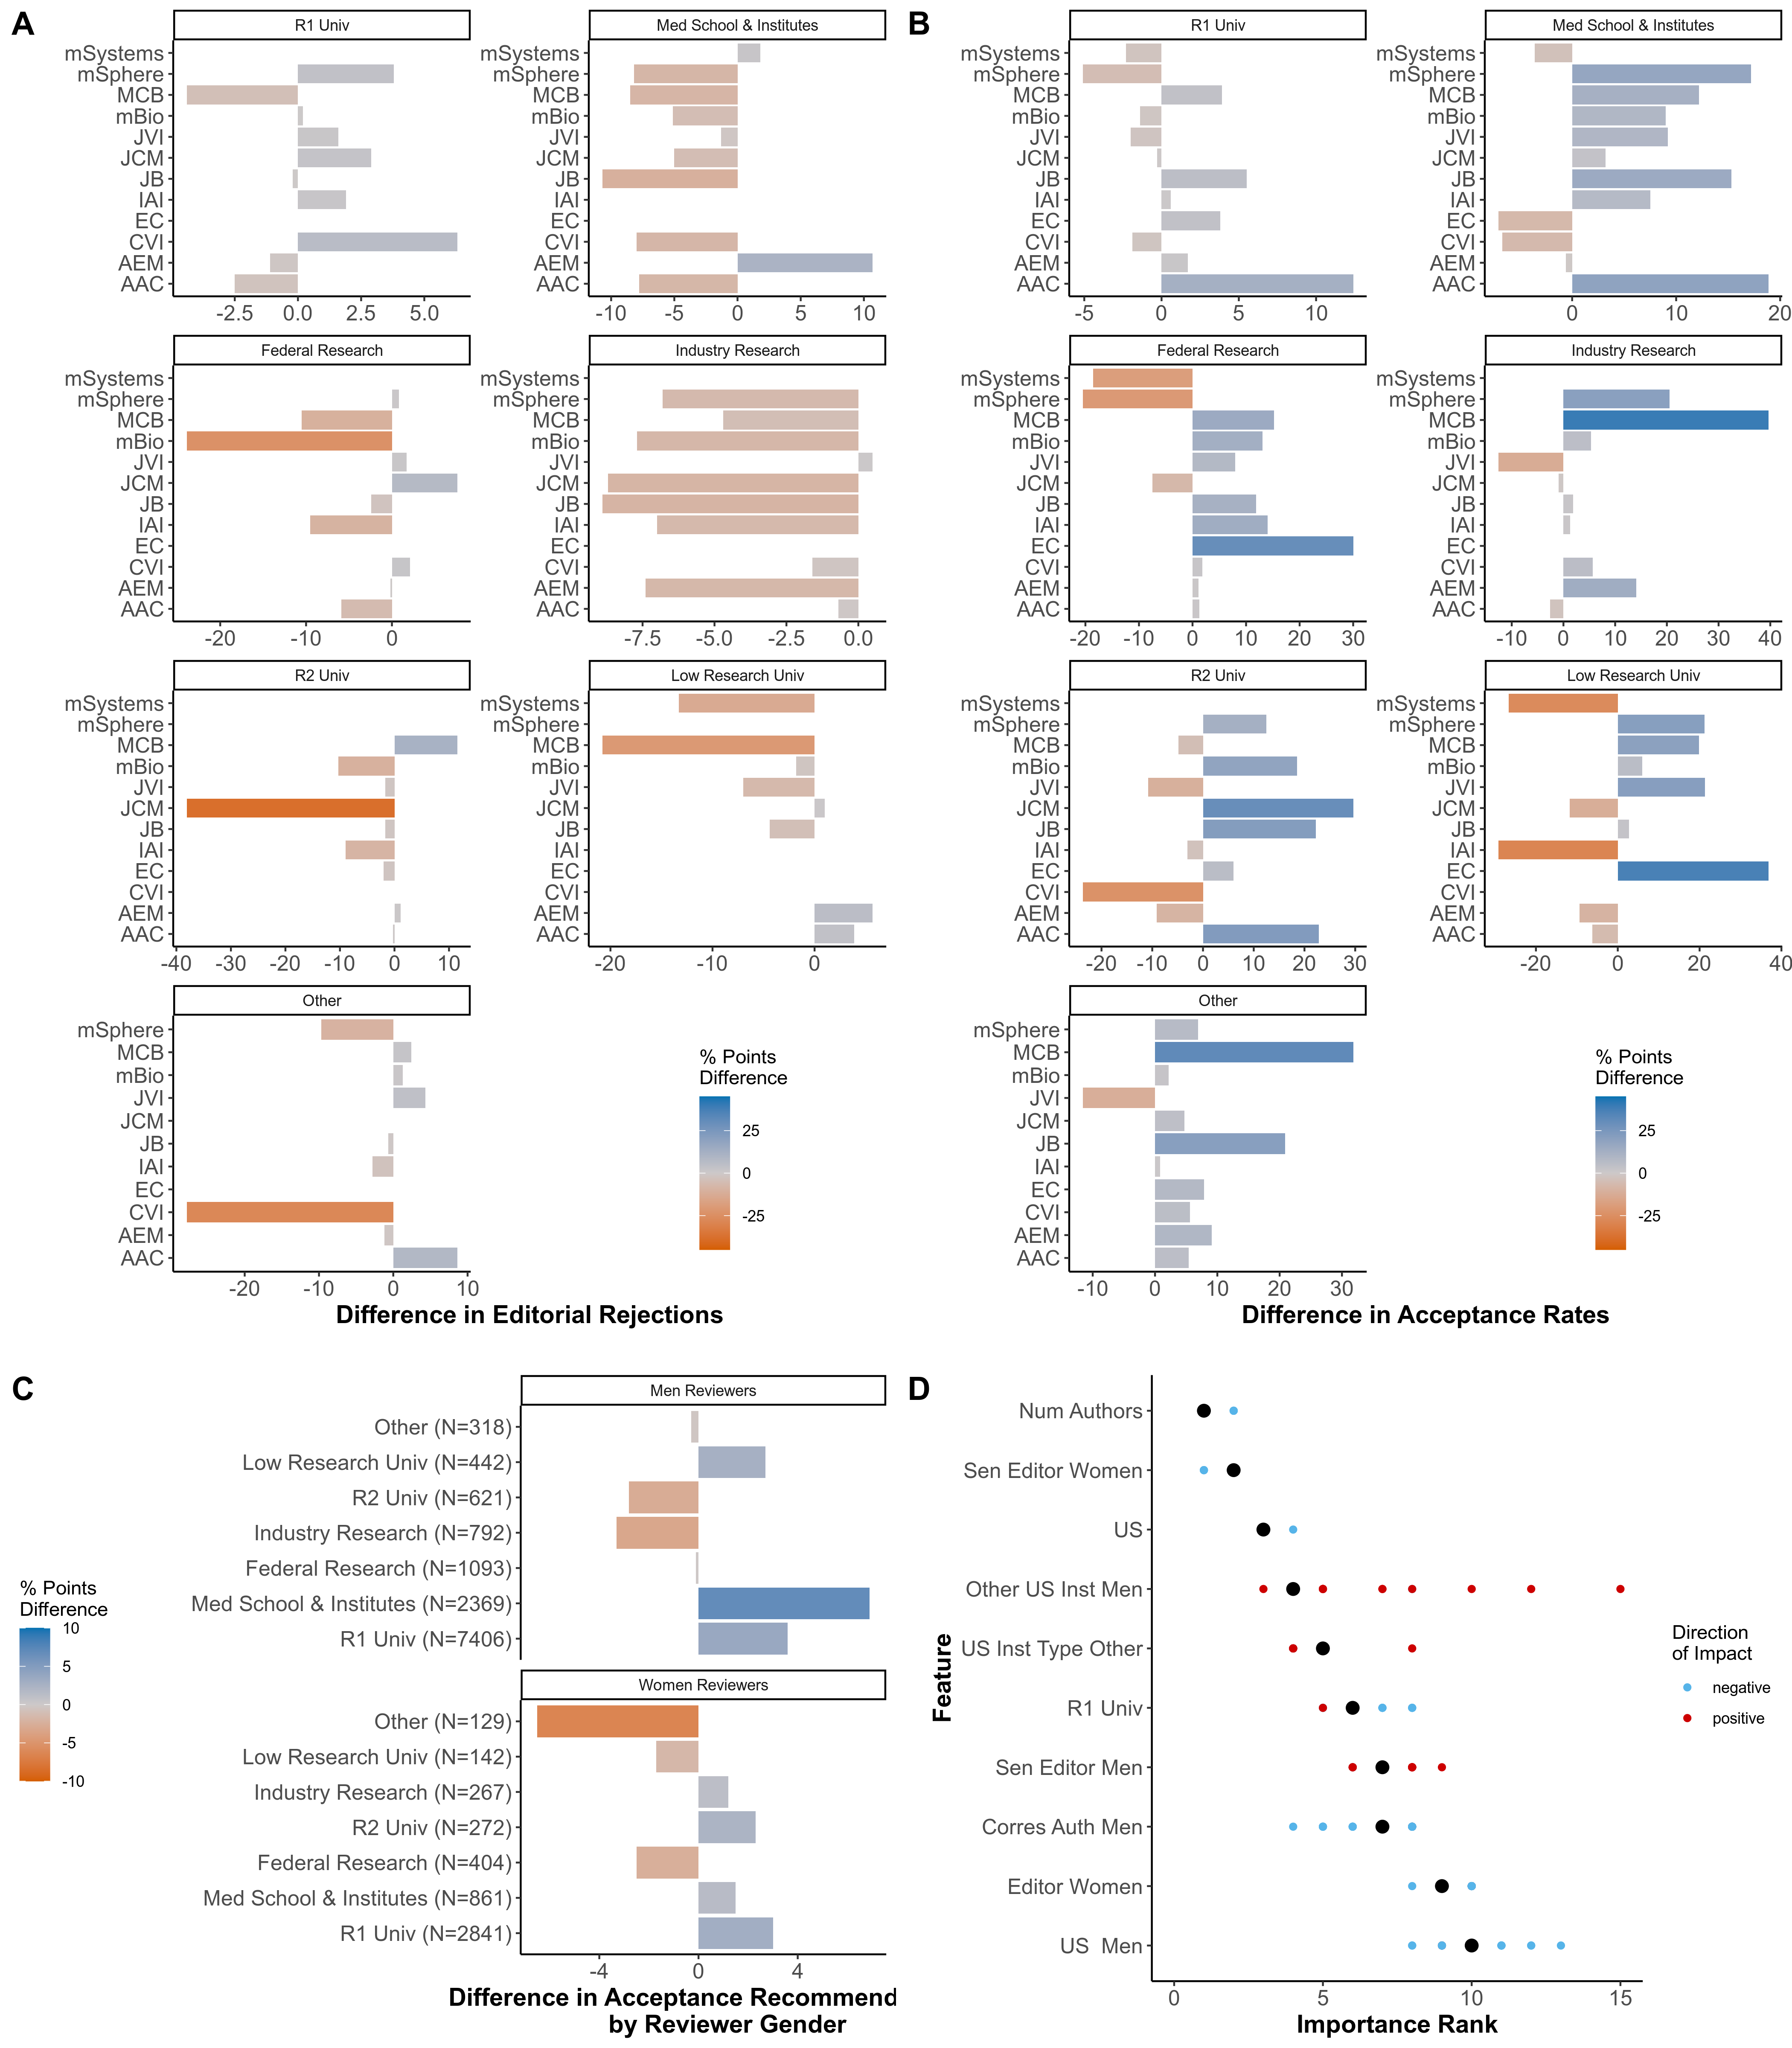
\includegraphics{Figure_S7.png}

Figure S7. The negative impact of each country on the overall gender
prediction of the validation dataset. Number indicates the total number
of names associated with each country.

\newpage

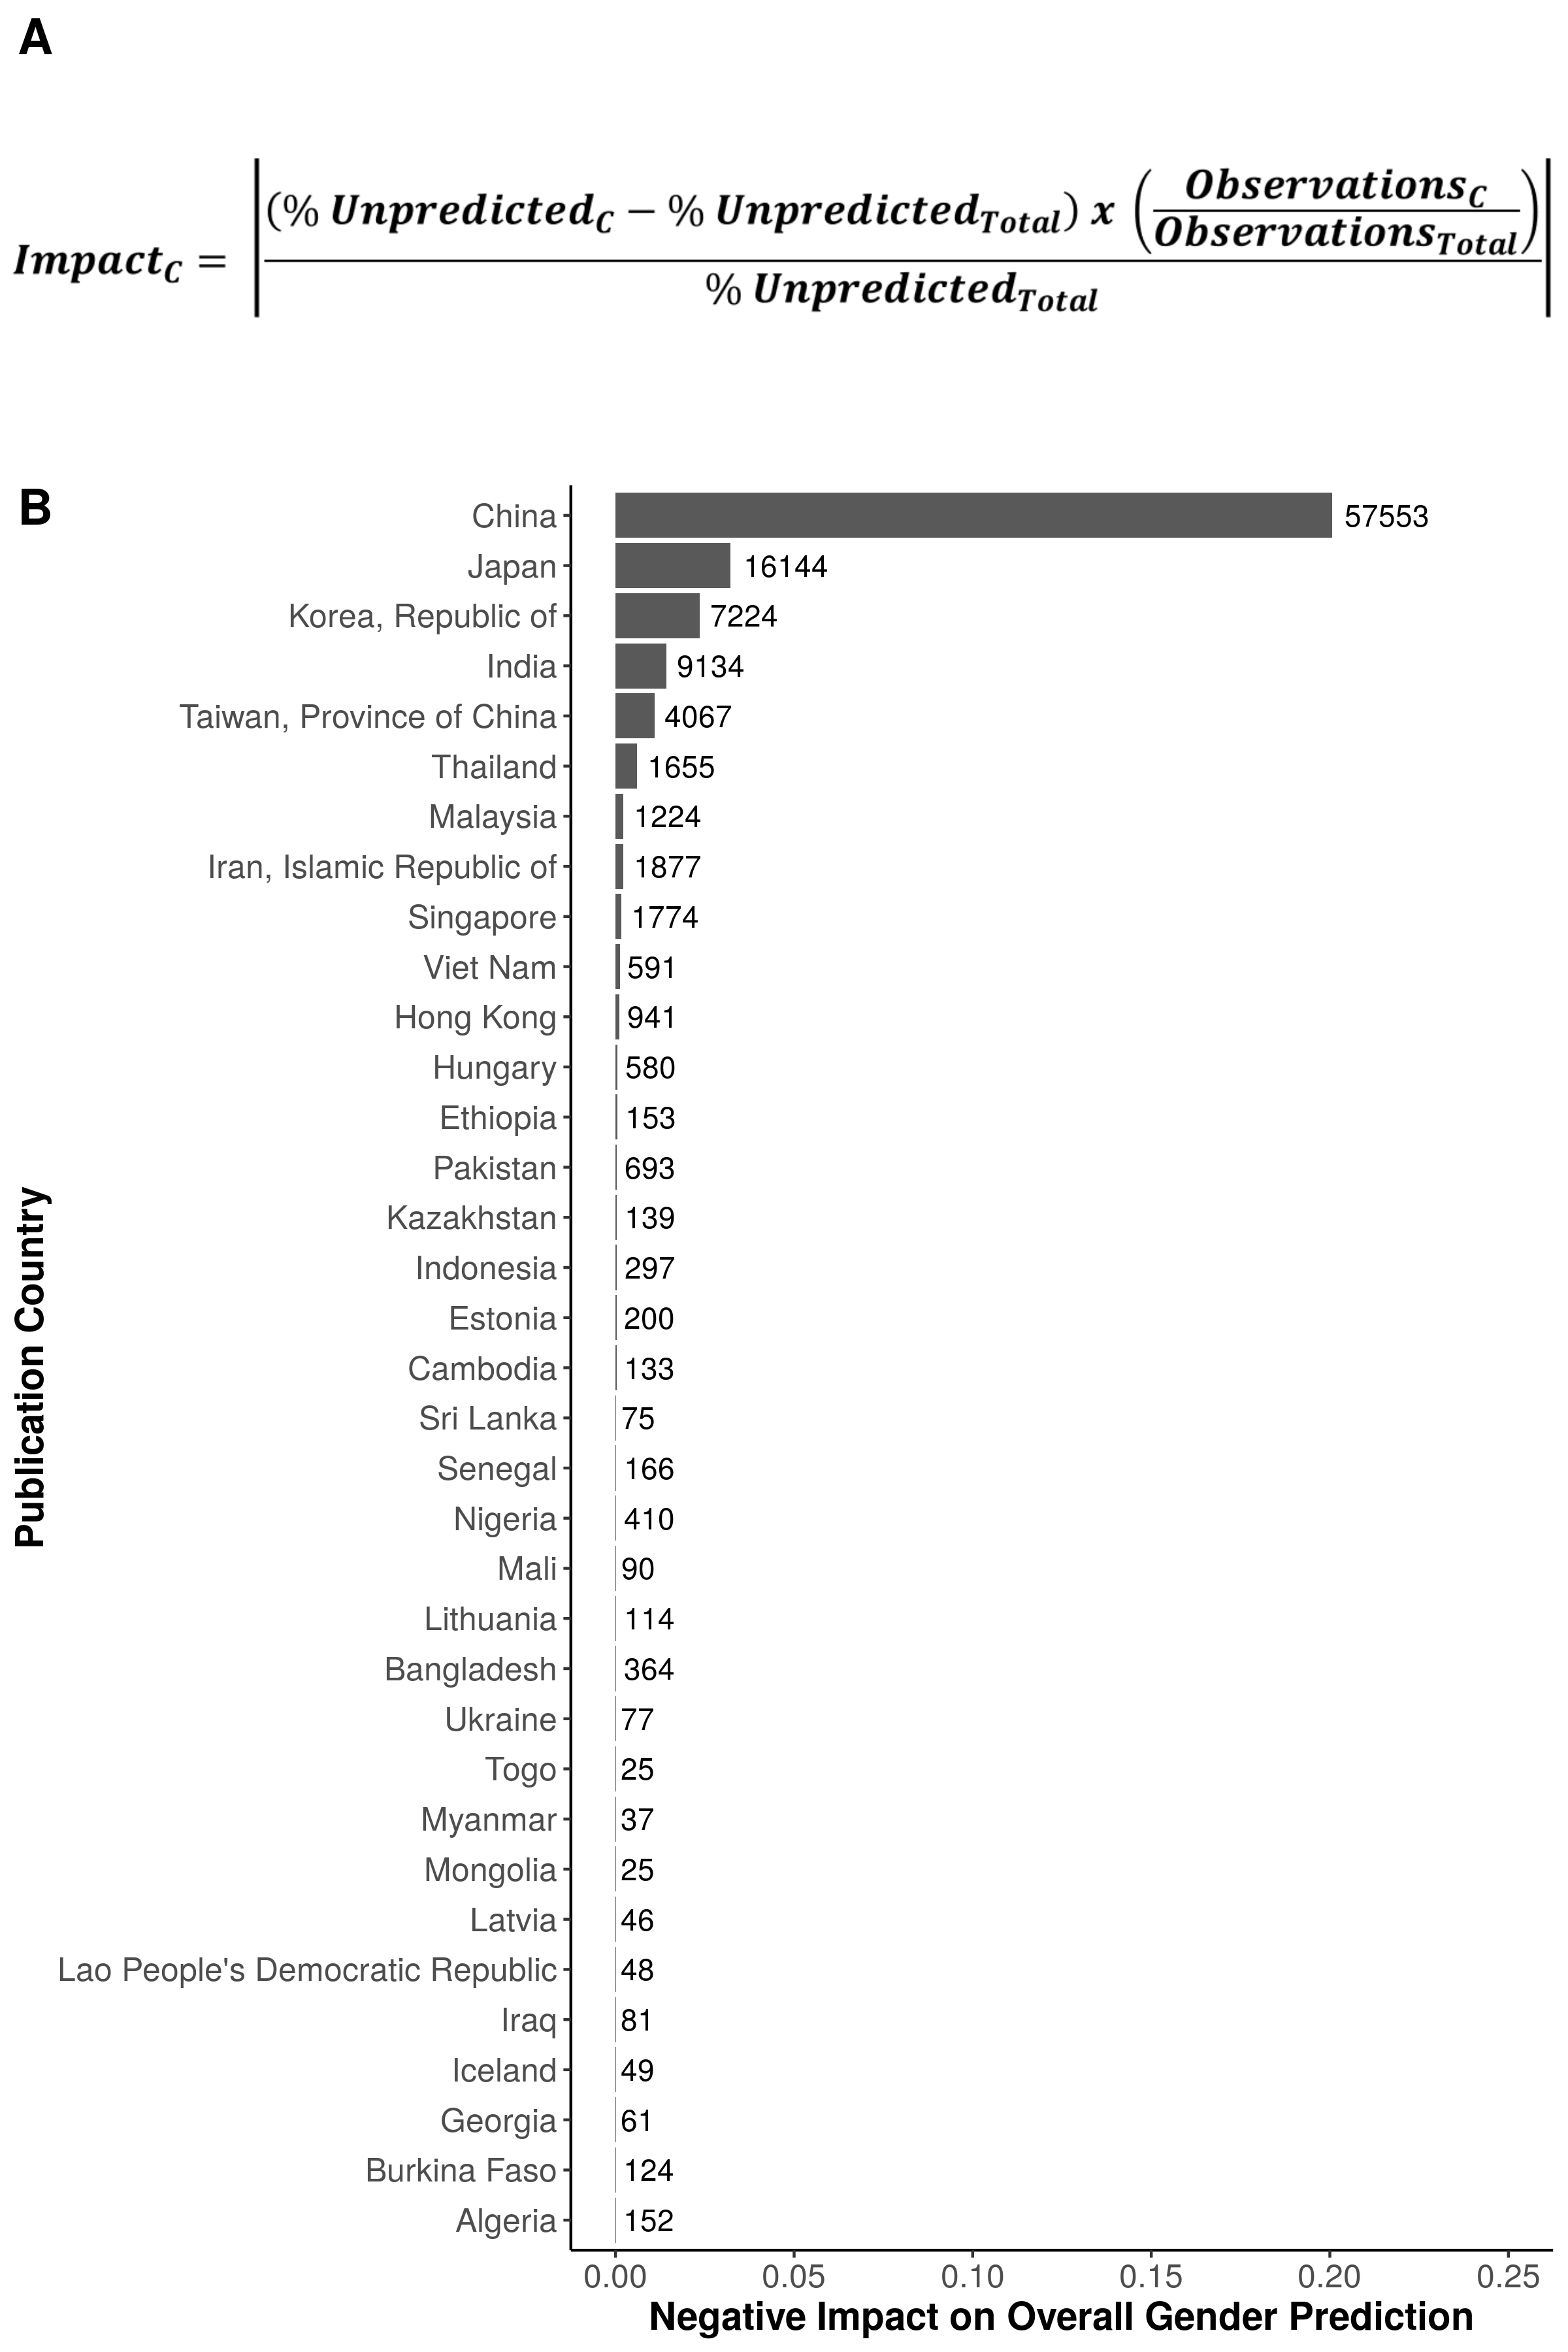
\includegraphics{Figure_S8.png}

Figure S8. The negative impact of each country on the overall gender
prediction of the full dataset. Number indicates the total number of
names associated with each country.


\end{document}
